\documentclass[12pt]{article}

%%%%%%%%%%%%%%%%%
% package
%%%%%%%%%%%%%%%%%
% layout
\usepackage[parfill]{parskip}
\usepackage{textcomp}
\usepackage[top=1in,left=.75in,right=.75in, bottom=1in]{geometry}
\usepackage{fancyhdr}
\usepackage{indentfirst}
% misc
\usepackage[utf8]{inputenc}
\usepackage{enumitem}
\usepackage{comment}
\usepackage{blindtext}
\usepackage{xspace}
\usepackage{tikz}
% \setlength{\marginparwidth}{2cm}
% \usepackage{todonotes}
% code listing
\usepackage{pythonhighlight}
\usepackage{listings}
% figure
\usepackage{graphicx}
% table
\usepackage{booktabs}
\usepackage{multirow}
\usepackage{array}
% color
\usepackage{xcolor}
% url style
\usepackage{url}
\usepackage{hyperref}
\definecolor{darkblue}{rgb}{0, 0, 0.5}
\hypersetup{colorlinks=true,citecolor=darkblue, linkcolor=darkblue, urlcolor=darkblue}
% cite style
\usepackage{natbib}
% box
\usepackage{mdframed}
\usepackage{tcolorbox}
% math
\usepackage{amsmath,amssymb,amsfonts,bbm,bm,mathtools}
% math: partial derivative
\usepackage{physics}
% math: theorem, definition
\usepackage{amsthm}
\newtheorem{theorem}{Theorem}[section]
\newtheorem*{theorem*}{Theorem}
\newtheorem{definition}{Definition}[section]
\newtheorem*{definition*}{Definition}
\newtheorem*{remark}{Remark}

%%%%%%%%%%%%%%%%%
% for table
%%%%%%%%%%%%%%%%%

\newcolumntype{C}[1]{>{\centering\arraybackslash}m{#1}}
\newcolumntype{L}[1]{>{\raggedright\arraybackslash}m{#1}}
\newcolumntype{R}[1]{>{\raggedleft\arraybackslash}m{#1}}

%%%%%%%%%%%%%%%%%
% math operator
%%%%%%%%%%%%%%%%%

\DeclareMathOperator*{\argmax}{arg\,max}
\DeclareMathOperator*{\argmin}{arg\,min}
% expectation
\DeclareMathOperator*{\E}{\mathbb{E}}
% gradient
\let\grad\relax % already defined in \usepackage{physics}
\DeclareMathOperator{\grad}{\nabla}
% bias
% \DeclareMathOperator*{\bias}{bias}


%%%%%%%%%%%%%%%%%
% new command
%%%%%%%%%%%%%%%%%
% remove spurious space around \left and \right
% e.g., you want var(.) rather than var (.)
\let\originalleft\left
\let\originalright\right
\renewcommand{\left}{\mathopen{}\mathclose\bgroup\originalleft}
\renewcommand{\right}{\aftergroup\egroup\originalright}
% parenthesis and brackets, nice size
\newcommand{\paren}[1]{\left(#1\right)} %( )
\newcommand{\bk}[1]{\left[#1\right]}  %brackets[ ]
\newcommand{\br}[1]{\left\{#1\right\}}  %braces { }
\newcommand{\ang}[1]{\left\langle#1\right\rangle} %angles < >
\newcommand{\set}[1]{\left\{#1\right\}} %{ }
% already defined in \usepackage{physics}
% \newcommand{\abs}[1]{\left|#1\right|} % L1 norm,
% already defined in \usepackage{physics}
% \newcommand{\norm}[1]{\left\|#1\right\|} % L2 norm


% misc
\newcommand{\bias}[1]{\mathrm{bias}\paren{#1}} % bias
\newcommand{\reals}{\mathbb{R}} % real number
\newcommand{\softmax}[1]{\mathrm{softmax}\paren{#1}}
\newcommand{\ind}[1]{\mathbbm{1}\bk{#1}}
\newcommand{\gives}{\;\,\Rightarrow\;\,}
% add parenthesis to exp
% \renewcommand{\exp}[1]{\mathrm{exp}\paren{#1}}
% math expression decoration
\newcommand{\ul}{\underline}
\newcommand{\ub}{\ensuremath{\underbrace}}
\newcommand{\ob}{\ensuremath{\overbrace}}
\newcommand{\ubk}{\ensuremath{\underbracket}}
\newcommand{\obk}{\ensuremath{\overbracket}}
% itemize
\newcommand{\bi}{\begin{itemize}}
\newcommand{\ei}{\end{itemize}}
% small circle for annotation
\newcommand{\mycircle}[1]{\raisebox{.5pt}{\textcircled{\raisebox{-.5pt} {\small #1}}}}
\newcommand{\ddd}{, \ldots, }


% Calculus, already defined in \usepackage{physics}
% 1st order derivative
% \newcommand{\dv}[2]{\frac{\mathrm{d} #1}{\mathrm{d} #2}}
% 1st order partial derivative 
% \newcommand{\pdv}[2]{\frac{\partial #1}{\partial #2}}

% Linear algebra
% redefine, \usepackage{physics}
\renewcommand{\rank}[1]{\mathrm{rank}\paren{#1}}
% redefine, \usepackage{physics}
\renewcommand{\tr}[1]{\mathrm{tr}\paren{#1}} % trace
% build a diagonal matrix from vector \diag{x_1,\ldots,x_n}; or extract a vector from the diagonal entries of a square matrix \diag{\ensuremath{\mathbf{X}}
\newcommand{\diag}[1]{\mathrm{diag}\paren{#1}} 
\newcommand{\inner}[2]{\left\langle #1, #2 \right\rangle} % <,>
% \span is already defined, so we use \Span instead
\newcommand{\Span}[1]{\mathrm{span}\paren{#1}}
\newcommand{\T}{^\top} % transpose
\newcommand{\inverse}{^{-1}} % inverse
\newcommand{\zero}{\ensuremath{\mathbf{0}}} % vector of zero
\newcommand{\Zero}{\ensuremath{\mathbf{O}}} % matrix of zero

% Probability
% redefine, \usepackage{physics}
\renewcommand{\var}[1]{\mathrm{var}\paren{#1}} % variance
\newcommand{\cov}[1]{\mathrm{cov}\paren{#1}} % covariance
\newcommand{\corr}[1]{\mathrm{corr}\paren{#1}} % correlation
\newcommand{\param}{;}
% independent and identically distributed
\newcommand{\iid}{\stackrel{\text{iid}}{\sim}}
% equal in distribution
\newcommand\deq{\stackrel{\text{d}}{=}}
% independent 
\newcommand{\indep}{\perp \!\!\! \perp}
% distribution names
% normal
\newcommand{\dn}[1]{\ensuremath{\mathcal{N}\paren{#1}}}
% multivariate normal, first argument is degree
\newcommand{\dmn}[2]{\ensuremath{\mathcal{N}_{#1}\paren{#2}}}
% use first four letter
\newcommand{\dunif}[1]{\ensuremath{\mathrm{Uniform}\paren{#1}}}
\newcommand{\dbern}[1]{\ensuremath{\mathrm{Bernoulli}\paren{#1}}}
\newcommand{\dmult}[1]{\ensuremath{\mathrm{Multinomial}\paren{#1}}}
\newcommand{\dbeta}[1]{\ensuremath{\mathrm{Beta}\paren{#1}}}
\newcommand{\dgumb}[1]{\ensuremath{\mathrm{Gumbel}\paren{#1}}}
% use first three letter
\newcommand{\dbin}[1]{\ensuremath{\mathrm{Binomial}\paren{#1}}}
\newcommand{\dexp}[1]{\ensuremath{\mathrm{Exponential}\paren{#1}}}
\newcommand{\dgeo}[1]{\ensuremath{\mathrm{Geometric}\paren{#1}}}
\newcommand{\dgam}[1]{\ensuremath{\mathrm{Gamma}\paren{#1}}}
\newcommand{\dpoi}[1]{\ensuremath{\mathrm{Poisson}\paren{#1}}}
\newcommand{\dchi}[1]{\ensuremath{\chi^2\paren{#1}}}
\newcommand{\dcat}[1]{\ensuremath{\mathrm{Categorical}\paren{#1}}}
\newcommand{\ddir}[1]{\ensuremath{\mathrm{Dirichlet}\paren{#1}}}
\newcommand{\dpar}[1]{\ensuremath{\mathrm{Pareto}\paren{#1}}}
\newcommand{\dcau}[1]{\ensuremath{\mathrm{Cauchy}\paren{#1}}}
\newcommand{\dwei}[1]{\ensuremath{\mathrm{Weibull}\paren{#1}}}
\newcommand{\dlog}[1]{\ensuremath{\mathrm{Logistic}\paren{#1}}}


% Information Theory
% Kullback–Leibler divergence
\newcommand{\KL}[2]{\mathrm{KL} \bk{#1\; \| \;#2} }

% bold lowercase: vector
\newcommand{\bolda}{\ensuremath{\mathbf{a}}}
\newcommand{\boldb}{\ensuremath{\mathbf{b}}}
\newcommand{\boldc}{\ensuremath{\mathbf{c}}}
\newcommand{\boldd}{\ensuremath{\mathbf{d}}}
\newcommand{\bolde}{\ensuremath{\mathbf{e}}}
\newcommand{\boldf}{\ensuremath{\mathbf{f}}}
\newcommand{\boldg}{\ensuremath{\mathbf{g}}}
\newcommand{\boldh}{\ensuremath{\mathbf{h}}}
\newcommand{\boldi}{\ensuremath{\mathbf{i}}}
\newcommand{\boldj}{\ensuremath{\mathbf{j}}}
\newcommand{\boldk}{\ensuremath{\mathbf{k}}}
\newcommand{\boldl}{\ensuremath{\mathbf{l}}}
\newcommand{\boldm}{\ensuremath{\mathbf{m}}}
\newcommand{\boldn}{\ensuremath{\mathbf{n}}}
\newcommand{\boldo}{\ensuremath{\mathbf{o}}}
\newcommand{\boldp}{\ensuremath{\mathbf{p}}}
\newcommand{\boldq}{\ensuremath{\mathbf{q}}}
\newcommand{\boldr}{\ensuremath{\mathbf{r}}}
\newcommand{\bolds}{\ensuremath{\mathbf{s}}}
\newcommand{\boldt}{\ensuremath{\mathbf{t}}}
\newcommand{\boldu}{\ensuremath{\mathbf{u}}}
\newcommand{\boldv}{\ensuremath{\mathbf{v}}}
\newcommand{\boldw}{\ensuremath{\mathbf{w}}}
\newcommand{\boldx}{\ensuremath{\mathbf{x}}}
\newcommand{\boldy}{\ensuremath{\mathbf{y}}}
\newcommand{\boldz}{\ensuremath{\mathbf{z}}}

% bold uppercase: matrix
\newcommand{\boldA}{\ensuremath{\mathbf{A}}}
\newcommand{\boldB}{\ensuremath{\mathbf{B}}}
\newcommand{\boldC}{\ensuremath{\mathbf{C}}}
\newcommand{\boldD}{\ensuremath{\mathbf{D}}}
\newcommand{\boldE}{\ensuremath{\mathbf{E}}}
\newcommand{\boldF}{\ensuremath{\mathbf{F}}}
\newcommand{\boldG}{\ensuremath{\mathbf{G}}}
\newcommand{\boldH}{\ensuremath{\mathbf{H}}}
\newcommand{\boldI}{\ensuremath{\mathbf{I}}}
\newcommand{\boldJ}{\ensuremath{\mathbf{J}}}
\newcommand{\boldK}{\ensuremath{\mathbf{K}}}
\newcommand{\boldL}{\ensuremath{\mathbf{L}}}
\newcommand{\boldM}{\ensuremath{\mathbf{M}}}
\newcommand{\boldN}{\ensuremath{\mathbf{N}}}
\newcommand{\boldO}{\ensuremath{\mathbf{O}}}
\newcommand{\boldP}{\ensuremath{\mathbf{P}}}
\newcommand{\boldQ}{\ensuremath{\mathbf{Q}}}
\newcommand{\boldR}{\ensuremath{\mathbf{R}}}
\newcommand{\boldS}{\ensuremath{\mathbf{S}}}
\newcommand{\boldT}{\ensuremath{\mathbf{T}}}
\newcommand{\boldU}{\ensuremath{\mathbf{U}}}
\newcommand{\boldV}{\ensuremath{\mathbf{V}}}
\newcommand{\boldW}{\ensuremath{\mathbf{W}}}
\newcommand{\boldX}{\ensuremath{\mathbf{X}}}
\newcommand{\boldY}{\ensuremath{\mathbf{Y}}}
\newcommand{\boldZ}{\ensuremath{\mathbf{Z}}}

% calligraphic uppercase: set
\newcommand{\mcA}{\ensuremath{\mathcal{A}}}
\newcommand{\mcB}{\ensuremath{\mathcal{B}}}
\newcommand{\mcC}{\ensuremath{\mathcal{C}}}
\newcommand{\mcD}{\ensuremath{\mathcal{D}}}
\newcommand{\mcE}{\ensuremath{\mathcal{E}}}
\newcommand{\mcF}{\ensuremath{\mathcal{F}}}
\newcommand{\mcG}{\ensuremath{\mathcal{G}}}
\newcommand{\mcH}{\ensuremath{\mathcal{H}}}
\newcommand{\mcI}{\ensuremath{\mathcal{I}}}
\newcommand{\mcJ}{\ensuremath{\mathcal{J}}}
\newcommand{\mcK}{\ensuremath{\mathcal{K}}}
\newcommand{\mcL}{\ensuremath{\mathcal{L}}}
\newcommand{\mcM}{\ensuremath{\mathcal{M}}}
\newcommand{\mcN}{\ensuremath{\mathcal{N}}}
\newcommand{\mcO}{\ensuremath{\mathcal{O}}}
\newcommand{\mcP}{\ensuremath{\mathcal{P}}}
\newcommand{\mcQ}{\ensuremath{\mathcal{Q}}}
\newcommand{\mcR}{\ensuremath{\mathcal{R}}}
\newcommand{\mcS}{\ensuremath{\mathcal{S}}}
\newcommand{\mcT}{\ensuremath{\mathcal{T}}}
\newcommand{\mcU}{\ensuremath{\mathcal{U}}}
\newcommand{\mcV}{\ensuremath{\mathcal{V}}}
\newcommand{\mcW}{\ensuremath{\mathcal{W}}}
\newcommand{\mcX}{\ensuremath{\mathcal{X}}}
\newcommand{\mcY}{\ensuremath{\mathcal{Y}}}
\newcommand{\mcZ}{\ensuremath{\mathcal{Z}}}
\newcommand{\mcnu}{\ensuremath{\mathcal{\nu}}}

% bold Greek symbol: parameter vector
\newcommand{\balpha}{\ensuremath{\boldsymbol{\alpha}}}
\newcommand{\bnu}{\ensuremath{\boldsymbol{\nu}}}
\newcommand{\bbeta}{\ensuremath{\boldsymbol{\beta}}}
\newcommand{\bxi}{\ensuremath{\boldsymbol{\xi}}}
\newcommand{\bXi}{\ensuremath{\boldsymbol{\Xi}}}
\newcommand{\bgamma}{\ensuremath{\boldsymbol{\gamma}}}
\newcommand{\bGamma}{\ensuremath{\boldsymbol{\Gamma}}}
\newcommand{\bdelta}{\ensuremath{\boldsymbol{\delta}}}
\newcommand{\bDelta}{\ensuremath{\boldsymbol{\Delta}}}
\newcommand{\bpi}{\ensuremath{\boldsymbol{\pi}}}
\newcommand{\bPi}{\ensuremath{\boldsymbol{\Pi}}}
\newcommand{\bepsilon}{\ensuremath{\boldsymbol{\epsilon}}}
\newcommand{\brho}{\ensuremath{\boldsymbol{\rho}}}
\newcommand{\bvarrho}{\ensuremath{\boldsymbol{\varrho}}}
\newcommand{\bzeta}{\ensuremath{\boldsymbol{\zeta}}}
\newcommand{\bsigma}{\ensuremath{\boldsymbol{\sigma}}}
\newcommand{\bSigma}{\ensuremath{\boldsymbol{\Sigma}}}
\newcommand{\btau}{\ensuremath{\boldsymbol{\tau}}}
\newcommand{\btheta}{\ensuremath{\boldsymbol{\theta}}}
\newcommand{\bvartheta}{\ensuremath{\boldsymbol{\vartheta}}}
\newcommand{\bTheta}{\ensuremath{\boldsymbol{\Theta}}}
\newcommand{\bupsilon}{\ensuremath{\boldsymbol{\upsilon}}}
\newcommand{\bUpsilon}{\ensuremath{\boldsymbol{\Upsilon}}}
\newcommand{\biota}{\ensuremath{\boldsymbol{\iota}}}
\newcommand{\bphi}{\ensuremath{\boldsymbol{\phi}}}
\newcommand{\bvarphi}{\ensuremath{\boldsymbol{\varphi}}}
\newcommand{\bPhi}{\ensuremath{\boldsymbol{\Phi}}}
\newcommand{\bkappa}{\ensuremath{\boldsymbol{\kappa}}}
\newcommand{\bchi}{\ensuremath{\boldsymbol{\chi}}}
\newcommand{\blambda}{\ensuremath{\boldsymbol{\lambda}}}
\newcommand{\bLambda}{\ensuremath{\boldsymbol{\Lambda}}}
\newcommand{\bpsi}{\ensuremath{\boldsymbol{\psi}}}
\newcommand{\bPsi}{\ensuremath{\boldsymbol{\Psi}}}
\newcommand{\bmu}{\ensuremath{\boldsymbol{\mu}}}
\newcommand{\bomega}{\ensuremath{\boldsymbol{\omega}}}
\newcommand{\bOmega}{\ensuremath{\boldsymbol{\Omega}}}
% need to write eta manually
% \newcommand{\beta}{\ensuremath{\boldsymbol{\eta}}

% basic color
% https://www.overleaf.com/learn/latex/Using_colours_in_LaTeX
\newcommand{\white}[1]{\textcolor{white}{#1}}
\newcommand{\black}[1]{\textcolor{black}{#1}}
\newcommand{\red}[1]{\textcolor{red}{#1}}
\newcommand{\green}[1]{\textcolor{green}{#1}}
\newcommand{\blue}[1]{\textcolor{blue}{#1}}
\newcommand{\cyan}[1]{\textcolor{cyan}{#1}}
\newcommand{\magenta}[1]{\textcolor{magenta}{#1}}
\newcommand{\yellow}[1]{\textcolor{yellow}{#1}}

%lst listing settings
\lstdefinestyle{custom}{
  belowcaptionskip=1\baselineskip,
  breaklines=true,
  frame=single,
  xleftmargin=\parindent,
  language=Python,
  showstringspaces=false,
  basicstyle=\footnotesize\ttfamily,
  keywordstyle=\bfseries\color{violet!60!purple},
  keywords=[2]{self, True, False},
  keywordstyle={[2]\ttfamily\color{blue!80!black}},
  commentstyle=\itshape\color{green!60!black},
  identifierstyle=\color{black},
  stringstyle=\color{orange},
}
\lstset{
basicstyle=\small,
escapechar=@,
style=custom,
upquote=true}
\usepackage{graphicx}

\title{Intro to AI 440, Assignment 1}
\author{Finn Jensen faj21, Jane McGrath ljm209, Andres Uribe aju24}
\date{Feb 09 2022}

\begin{document}
\maketitle
\thispagestyle{fancy}

\maketitle

%%%%%%%%%%%%%%%%%%%%%%%%%%%%%%%%%%%%%%%% P1
\section*{Question 1} 
%Write down your answers ... %
{
{\bf a)}
\\
For this project, the python tkinter library was used in the visualization, called in the files "draw.py" and "griddisplay.py". Additionally, the methods "readin.py", "Vertex.py", and "Graph.py" were written in order to create the underlying vertices and graphs in this project.
\\
\\
Eight neighbor grids are represented by a model that uses a Graph class and a Vertex class.
\\
\\
The Vertex class represents nodes on the eight neighbor grid and stores their g, h, and f-values. Vertex objects are identified by a unique key in the form “$x|y$”. The class also maintains a neighbors dictionary with neighboring vertices as the key and that edges weight as the value.
\\
\\
The graph class maintains a list of all of the participating vertices, the starting and goal vertices and a dictionary that keeps track of which cells are blocked and unblocked.
\\
\\
These grids interact with the front end visualization (which consists of "griddisplay.py" and "draw.py") by providing a Graph object that represents the eight neighbor grid with a start and goal node. The path is generated later by the A* or Theta* algorithm class.
\\
\\
The file “griddisplay.py” contains a class “Display”. A Display object is created with a graph, an integer "scale", and an integer "radius". The "scale" integer takes care of the visibility of the displayed grid, and the "radius" integer determines the size of the average vertex. The Display object will have its own Tkinter root window, a frame, a canvas, two scrollbars (one for horizontal scrolling and one for vertical scrolling), and it will also configure all these features (the window, the canvas, the scrollbars). “Display” also contains the methods “coordinate\_producer”, “display\_info”, and “bind\_canvas”.
\\
\\
The “coordinate\_producer” method only takes a Display object. First, it obtains the start and goal vertices with the graph methods “start\_node\_key” and “goal\_node\_key”, scales them up according to the Display object’s “scale” attribute, and then calls the “points” method (from "draw.py") to draw them with a larger radius in the color “red”. The “coordinate\_producer” method then iterates over each vertex in the graph, and then over each neighbor of that vertex. It obtains the coordinates of every vertex using the Vertex method "getKeyCoordinates", and then calls “points\_and\_lines” (from "draw.py"). Each vertex will have the tag “vertex”. Once every vertex and its neighbors have been drawn, this method is finished.
\\
\\
Then, the “bind\_canvas” method will use tkinter’s “tag\_bind” method to bind all objects that are tagged with “vertex” to the event of a mouse click, and to the “display\_info” method. When a vertex (tagged “vertex”) is clicked on, “display\_info” is called. It obtains the x and y coordinates of the mouse’s position, and then iterates over the vertices in the Display object’s graph. The vertices that have been drawn on the canvas have a certain radius determined by the Display object’s vertex\_radius; they have also been scaled up according to the Display object’s scale attribute. So, for each vertex in the graph, this method checks if the mouse-click-coordinates are within a range of “vertex\_radius” of that original vertex’s coordinates. It obtains the original vertex coordinates through "getKeyCoordinates", of course. It scales the value of the original vertex by the Display object's attribute “scale” to do so. The exact coordinates which correspond to a vertex are very difficult to hit, so this allows the entire drawn region that a vertex occupies to be clicked on instead. If the coordinates are within range, this method then obtains the g-, h-, and f-values of the vertex, and prints them to the terminal, along with the vertex's coordinates.
\\
\\
“draw.py” contains very simple methods: “points”, “lines”, “draw\_path”, and “points\_and\_lines”. The method “points\_and\_lines” is generally called first, and takes two sets of coordinates (four integers) and a Display object (defined in “griddisplay.py”) as its parameters. With these parameters, it calls the “lines” and “points” methods. The “lines” method simply uses the “create\_line” method from tkinter, and colors it with the passed fill color. It obtains the Display object’s canvas to create this line, with the passed coordinates.
\\
\\
Unlike the other methods, the “points” method needs a specific canvas and radius passed, along with an x coordinate, a y coordinate, a string for a tag, and a string for a fill color. With the radius provided, “points” calculates the appropriate integers to pass to tkinter’s “create\_oval” method, which will then fill the circle created with the provided fill, and tag it with the provided tag, on the provided canvas.
\\
\\
The "points" method is called by the Display class once specifically for the start and goal vertices, which must be larger than the average vertex. The need to make these vertices larger is the reason why the "points" method currently does not take a Display object as a parameter, and instead requires a specific canvas and a specific radius.
\\
\\
These three methods, “points\_and\_lines”, “points”, and “lines”, are all in charge of drawing the vertices and edges of the graph. The method “draw\_path”, on the other hand, can be called with the path that the A* family algorithms return. It takes a Display object, the path which an algorithm returns, and some fill color. The "draw\_path" method iterates over each pair of coordinates in the path that is passed to it, which are scaled up according to the Display object's scale attribute, and then calls the "lines" method on these scaled-up coordinates.
\\
\\
When the appropriate graph is displayed, the “start” and “goal” vertices should appear outlined in red, and the path that an algorithm takes should also be in red. When clicking on a vertex, a user should take care to click precisely within the filled-in black part of the vertex, and not outside or on any lines. The “draw\_path” method is called after the vertices have all been drawn, and so the line it draws will appear above the vertices of the graph. Such regions will not allow for “display\_info” to be called appropriately, because the lines are essentially obscuring the click-able portions of the vertices. 
\\
\\
\\
{\bf b)}
\\
The following is a manual computation of the shortest grid path for the problem from Figure 7:
\\
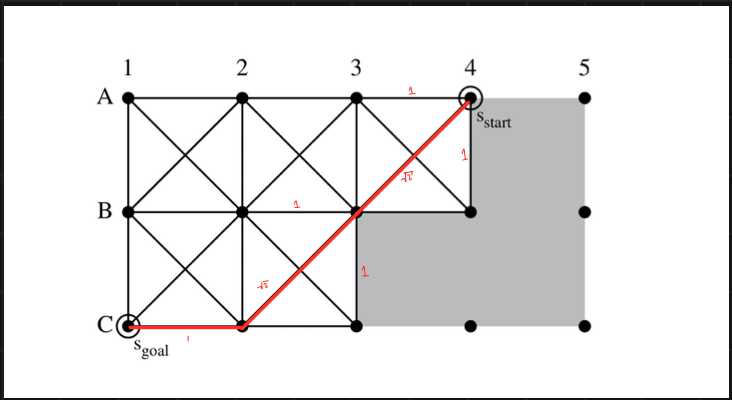
\includegraphics{s_grid_man.png}
\\
The following is a manual computation of the shortest any-angle path for the problem from Figure 7:
\\
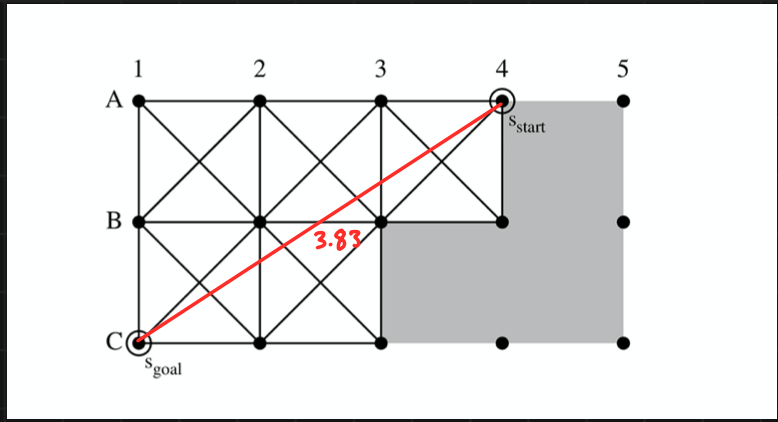
\includegraphics{s_any_man.png}
\\
The following images depict a manually computed trace of A* with the h-values from Equation 1:
\\
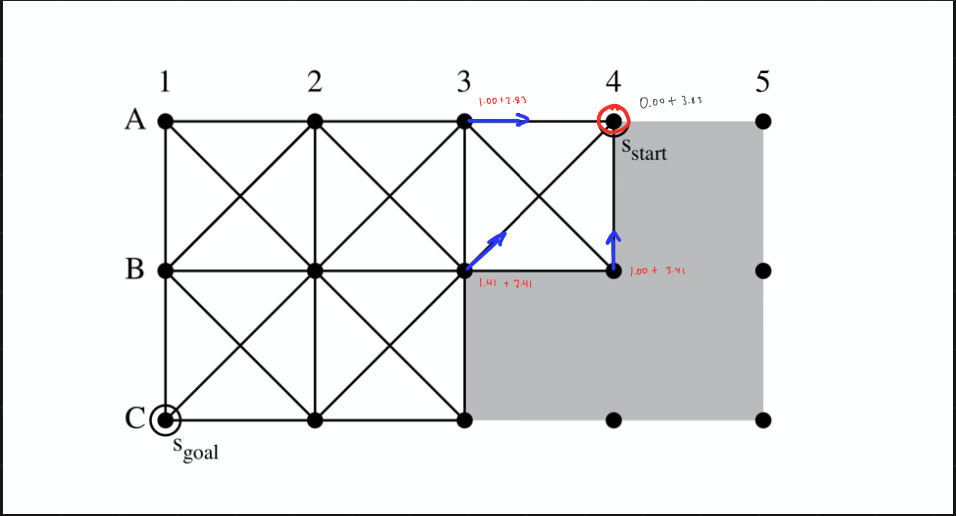
\includegraphics{s_grid_a_1.png}
\\
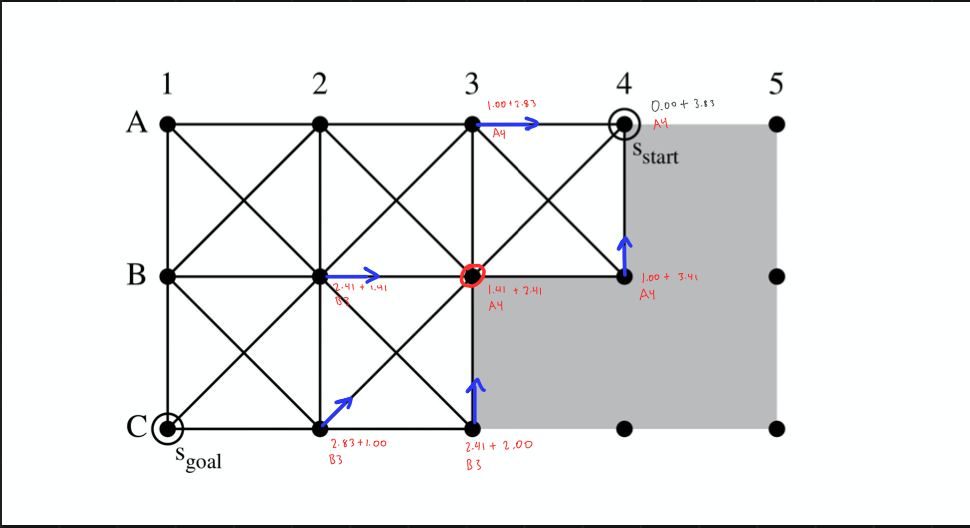
\includegraphics{s_grid_a_2.png}
\\
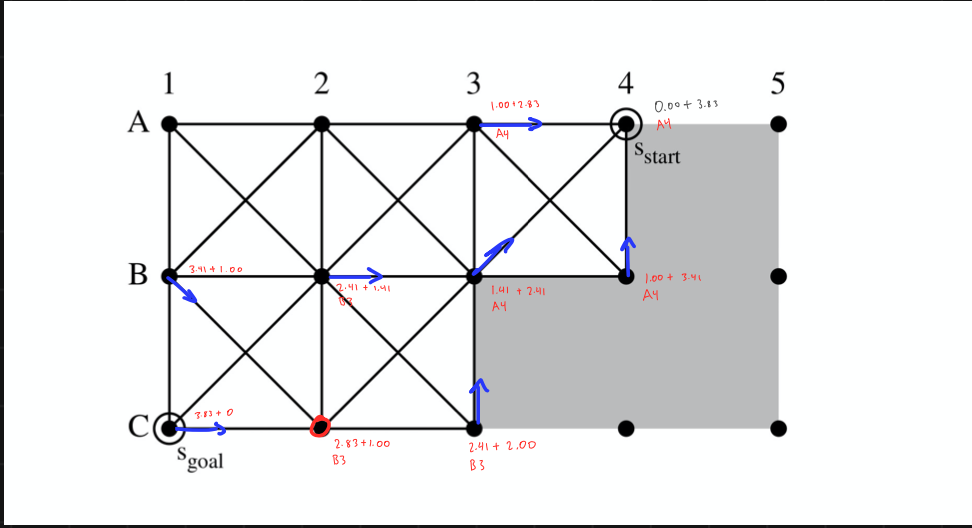
\includegraphics{s_grid_a_3.png}
\\
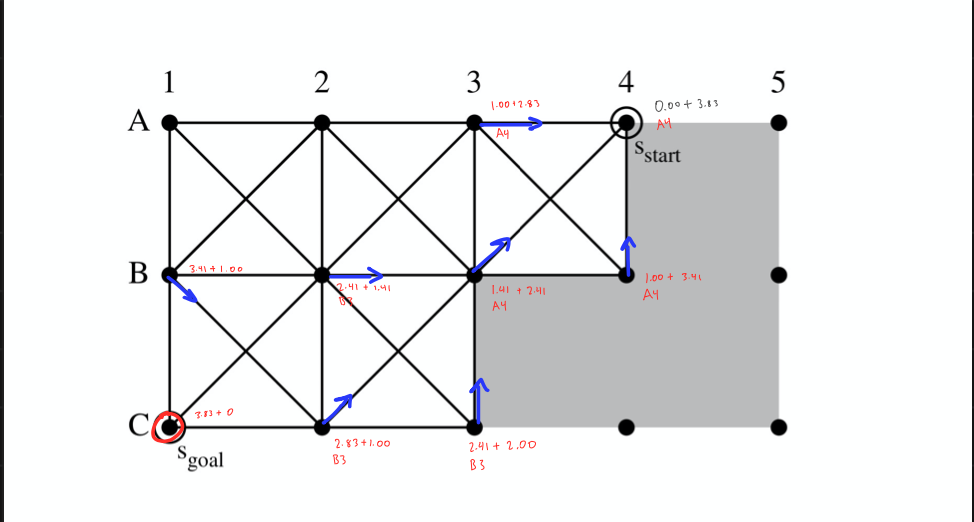
\includegraphics{s_grid_a_4.png}
\\
The following are a manually computed trace of Theta* with the h-values $h(s) = s(s, s_{goal})$
\\
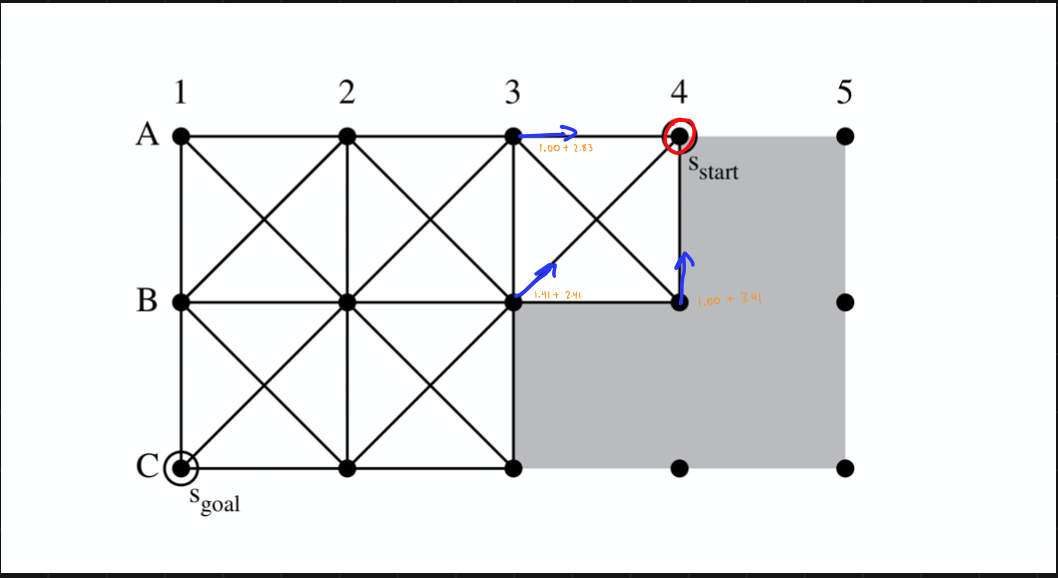
\includegraphics{s_grid_t_1.png}
\\
Note that the f-values are displayed rounded to 2 decimal places. At this step the real f-values for A2 and B2 are equal, so a node is chosen by tie-breaking.
\\
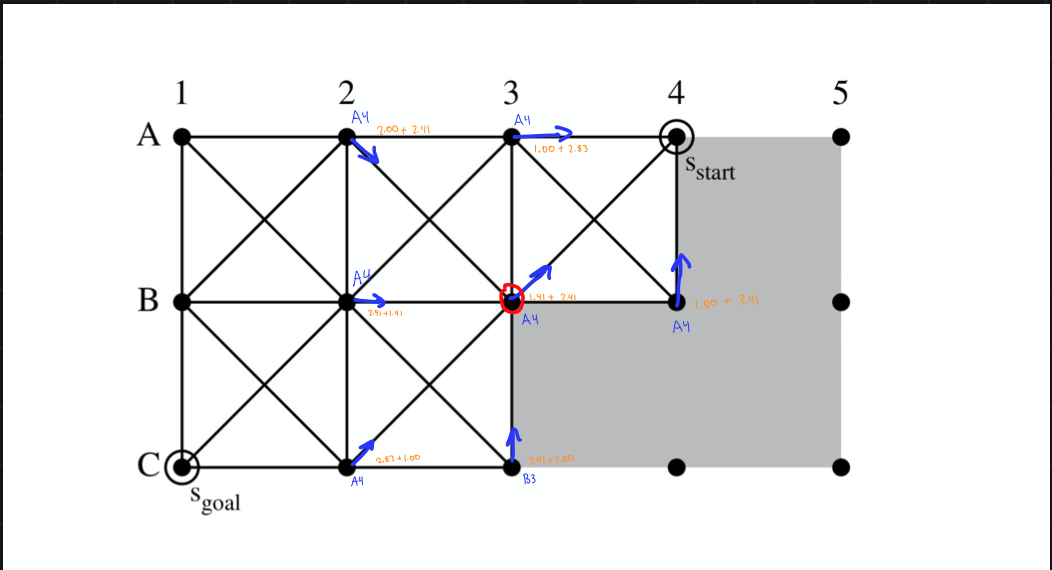
\includegraphics{s_grid_t_2.png}
\\
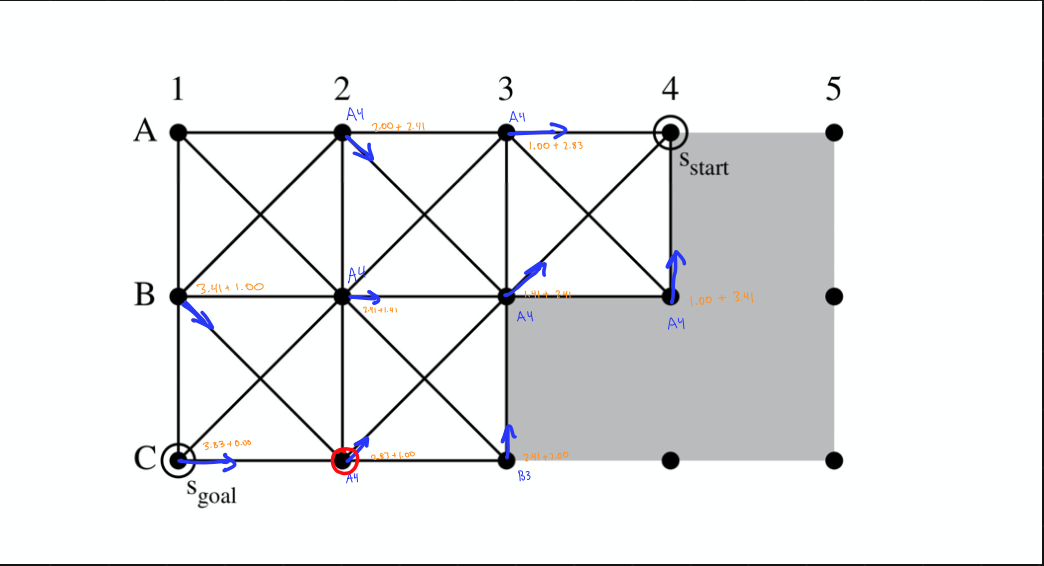
\includegraphics{s_grid_t_3.png}
\\
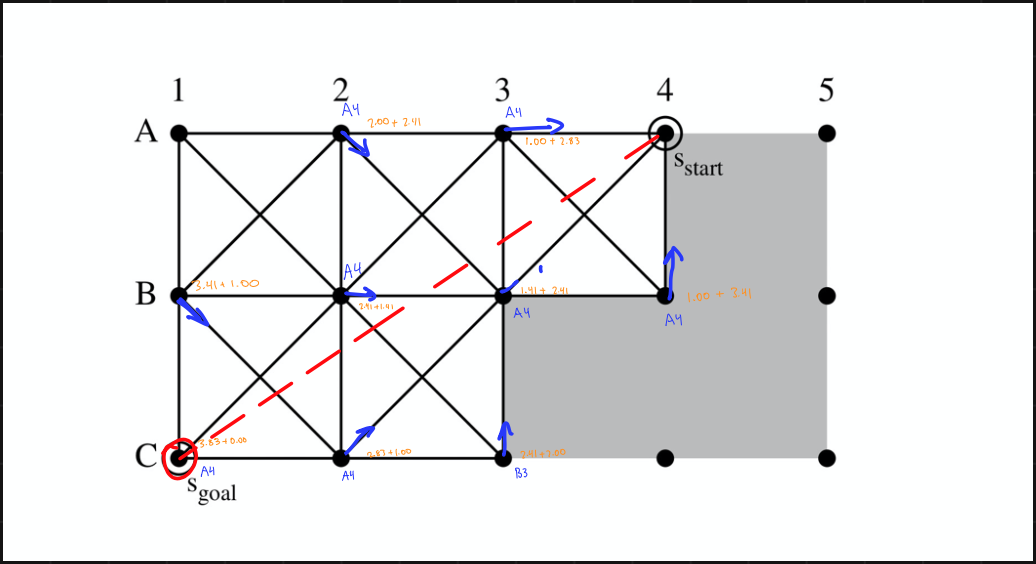
\includegraphics{s_grid_t_4.png}
\\
\\
\\
{\bf c)}
\\
A* and Theta* are implemented as classes with a main method closely following their respective pseudocodes.
\\
\\
The AStar class is interacted with through its main method. It accepts a graph object as a parameter and then when the main method is run $[AStar(graph).main()]$ it returns the shortest path as a list of nodes from start node to goal node. AStar implements $main$, $g$, $h$, $shortest\_path$, and $UpdateVertex$.
\\
\\
The AStar class also uses heapq from python in order to implement a heap which is then used throughout the class, with the fringe and closed list.
\\
\\
In shortest\_path(end\_node), given the final node after running, A* traces the path to that node through its parents, and returns a reversed list.
\\
\\
Note: All other methods are implemented exactly as described in the project description.
\\
\\
\\
{\bf d)}
\\
In order to get Theta* working, there were some slight changes that had to be made to the A* algorithm. 
\\
\\
The first change occurred in the updateVertex() method. On top of the path that was considered by A*, Theta* also considered the following path: start vertex to parent of vertex s, and parent of vertex s to successor vertex s'. This was achieved by computing the straight line distance between the parent of vertex s and its successor s'.
\\
\\
Theta* also checks if this straight line is even possible by checking whether it crosses through a blocked cell or not. This was achieved in the LineOfSight() method by calling a helper method cellsBlocked(). This method uses a dictionary where the key is a vertex and the value is 0 or 1, where 0 and 1 correspond to an unblocked and a blocked cell, respectively.
\\
\\
\\
{\bf e)}
\\
The A* algorithm must be consistent in order to guarantee that it finds the shortest grid paths. Therefore,
\[h(s) = \sqrt{2} * min(|s^x - s^x_{goal}|, |s^y - s^y_{goal}|) + max(|s^x - s^x_{goal}|, |s^y - s^y_{goal}|) - min(|s^x - s^x_{goal}|, |s^y - s^y_{goal}|)\]
must be consistent for A* to find the shortest grid paths.
\\
\\
For h(s) where s=goal, h(s) must be zero. This means
\[h(s) = sqrt[2] * min(0, 0) + max(0, 0) - min(0, 0)\]
Assuming h(s) is indeed consistent, $h(s) \leq c(s, s') + h(s')$ must be true.
\\
\\
If s' were the goal vertex, and s is a vertex one step away, it could be said that $h(s) \leq c(s, s_{goal}) + h(s_{goal})$
\\
\\
However, $h(s_{goal})$ is zero, so $h(s) \leq c(s, s_{goal})$
\\
\\
This means that for h(s), $h(s) = \sqrt{2} * min(|s^x - s^x_{goal}|, |s^y - s^y_{goal}|) + max(|s^x - s^x_{goal}|, |s^y - s^y_{goal}|) - min(|s^x - s^x_{goal}|, |s^y - s^y_{goal}|)$ is still less than the straight line distance between the current vertex and the goal vertex. This sort of heuristic ensures that the current vertex should indeed be chosen, being one step away from the goal.
\\
\\
s' is a vertex which is a successor to vertex s. Assume $s' = s_{goal}$, and that the heuristic is consistent.
\\
\\
Then it can be said that $g(s') = g(s) + c(s, a, s')$
\\
\\
Additionally, $f(s') = g(s') + h(s')$
\\
\\
It can also be said that $f(s') = g(s') + h(s') = g(s) + c(s, a, s') + h(s')$, which is all greater than $g(s) + h(s) = f(s)$
\\
\\
However, $h(s_{goal})$ is zero.
\\
\\
This means that $g(s') = g(s) + c(s, a, s')$ and that $f(s') = g(s') + 0$, so $g(s') = f(s')$
\\
\\
It can then be said that
\[f(s') = g(s') = g(s) + c(s, a, s') \geq g(s) = f(s)\]
\[f(s') = f(s) + c(s, a, s') \geq f(s)\]
\[f(s') = f(s) + c(s, a, s')\]
Because f(s') is a successor to s, and because f(s) is less than f(s'), this proves the values of f(s) on any path are nondecreasing.
\\
\\
}

\end{document}
